\ylDisplay{Kärbes peeglites} % Ülesande nimi
{Tundmatu autor} % Autor
{lõppvoor} % Voor
{2014} % Aasta
{P 7} % Ülesande nr.
{3} % Raskustase
{
% Teema: Valgusõpetus
\ifStatement
Kahe tasapeegi vaheline nurk on $120$$^{\circ}$  (vt joonist). Punktis $A$ asub vaatleja ning mööda sirget $s$ lendab edasi ja tagasi kärbes. Kärbse teatud asukohtade korral näeb vaatleja peeglites kahte kärbse kujutist. Tähistage sirgel $s$ see piirkond, mil tekib kaks kujutist.
\begin{center}
	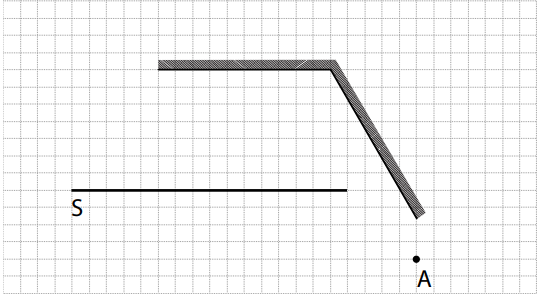
\includegraphics[width=0.5\linewidth]{2014-v3p-07-yl.PNG}
\end{center}
\fi
\ifHint
Sobiva piirkonna leidmisel tuleb arvestada kõikide võimalike piiripealsete punktidega ning leida nendes olevad kiirte peegeldumisnurgad.
\fi
\ifSolution
\begin{center}
	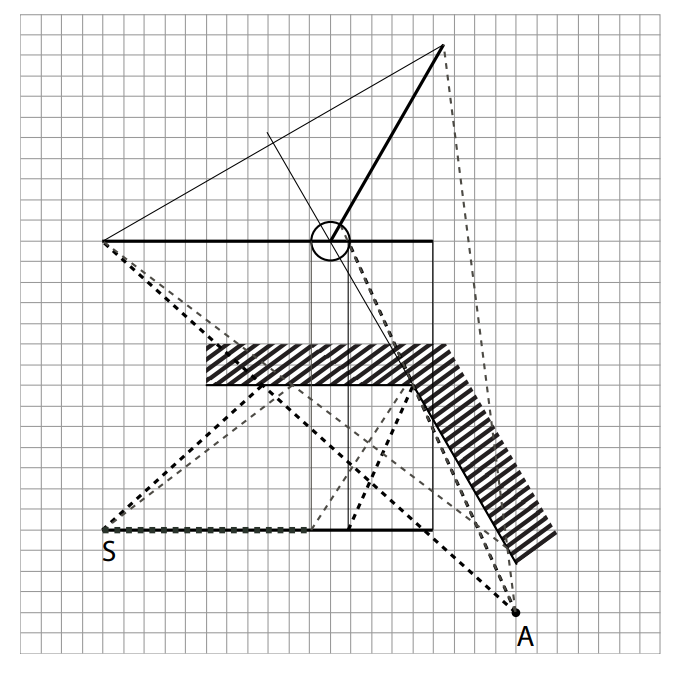
\includegraphics[width=0.5\linewidth]{2014-v3p-07-lah.PNG}
\end{center}
\fi
}
